\section{Κατηγορίες χρηστών} \label{section:3-2-user-categories}

Κατηγορίες:
1. Επισκέπτες
2. Εγγεγραμμένοι χρήστες
3. Δημιουργοί κοινοτήτων ?

\subsection{Πρώτο μέρος} \label{subsection:4-4-first-part}

Όπως προειπώθηκε, το πρώτο μέρος της πλατφόρμας θα είναι ανοιχτό σε όλους. Ωστόσο, οι χρήστες του μπορούν να διακριθούν
στις εξής δύο κατηγορίες:

\begin{itemize}
    \item Έμπιστα μέλη του δικτύου (trusted users)
    \item Μη έμπιστα μέλη  (untrusted users)
\end{itemize}

Βασική διαφορά των δύο κατηγοριών είναι πως ενώ οι trusted users θα αποζημιώνονται αυτόματα από το (ενν. φορτισμένο)
smart contract και άρα θα είναι απαλλαγμένοι από τέλη, οι δεύτεροι θα πρέπει να καταβάλουν μόνοι τους τα τέλη τους
(fees) για κάθε ενέργεια (π.χ. posting).

Η εμπιστοσύνη ενός χρήστη (trust) μπορεί να οριστεί ως ένας ακέραιος αριθμός με κάποιο κατώφλι, πάνω από το οποίο ο
χρήστης θα θεωρείται trusted. Το trust θα μπορεί να αυξομειώνεται ανά πάσα στιγμή, με τους χρήστες να δίνουν και να
παίρνουν βαθμούς trust σε/από άλλους.

Αξίζει να σημειωθεί επίσης ότι επειδή όλες οι συναλλαγές καταγράφονται, είναι δυνατό να υπολογιστεί το συνολικό ποσό του
Ethereum που έχει ξοδέψει ένας common user μέχρι να γίνει trusted και έτσι μπορεί σταδιακά να του επιστραφεί μέσω του
contract. Αυτό δίνει κίνητρο στους χρήστες να διατηρούν σωστή συμπεριφορά και να συμβάλλουν θετικά στην πλατφόρμα.

\subsection{Δεύτερο μέρος}

Για το δεύτερο μέρος της πλατφόρμας, οι χρήστες του μπορούν να διακριθούν στις εξής κατηγορίες: 

\begin{itemize}
    \item Πιστοποιημένα μέλη του Α.Π.Θ. (verified users)
    \item Μη πιστοποιημένα μέλη του Α.Π.Θ. (untrusted users)
\end{itemize}

Σχετικά με το δικαίωμα ψήφου για αυθεντικές δημοκρατικές αποφάσεις σχετικές με το ΑΠΘ, αυτό θα το έχουν μόνο οι verified
χρήστες του δικτύου. Οι verified χρήστες θα μπορούν επιπλέον να αλληλεπιδρούν με την πλατφόρμα εξαρχής χωρίς την
καταβολή τελών (θα ξεκινάνε ως trusted), πράγμα βέβαια που δε σημαίνει ότι χάνοντας trust δε θα μπορούν να χάσουν αυτό
το προνόμιο.

\subsection{Σύνοψη χρηστών}

Συμπερασματικά προκύπτουν τέσσερις διακριτές κατηγορίες χρηστών με ξεχωριστά δικαιώματα όπως φαίνεται στο παρακάτω
σχήμα (σχήμα \ref{figure:3-2-use-categories-diagram}):

\begin{figure}[H]
    \centering
    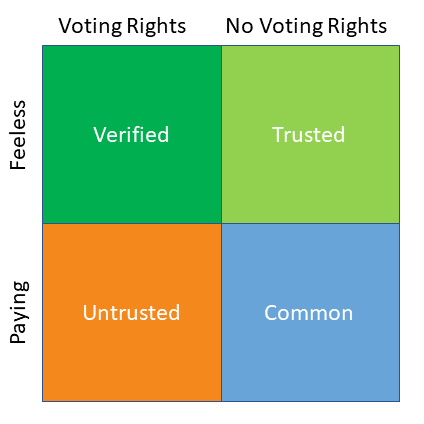
\includegraphics[width=0.6\textwidth]{assets/figures/chapter-3/user_categories}
    \caption{Κατηγορίες χρηστών}
    \label{figure:3-2-use-categories-diagram}
\end{figure}
